\themaG
\graphicspath{{../Ch5_Le_cercle/Images/}}

\chapter{Cercles et disques}
\label{C12}


%%%%%%%%%%%%%%%%%%%%%%%%%%%%%%%%%%%%%%%%%%
\begin{prerequis}[Connaissances et compétences abordées]
   \begin{itemize}
      \item Reconnaître, nommer le cercle (comme ensemble des points situés à une distance donnée d’un point donné), le disque.
      \item Vocabulaire associé au cercle et à leurs propriétés : centre, rayon, diamètre, milieu.
   \end{itemize}
\end{prerequis}

\vfill

\begin{debat}[Débat : les crop circle] 
   Un {\bf cercle de culture} (traduction de {\bf crop circle}), ou {\bf agrogramme} ou encore {\bf agroglyphe} est un très grand motif ou un ensemble de motifs géométriques réalisé dans un champ de céréales en couchant les épis au sol, ils sont apparus pour la première fois dans les années 1970. Ces formes impressionnantes sont visibles depuis le ciel. Pendant plusieurs années, on croyait que leur origine était extra-terrestre jusqu'à ce que l'on découvre leur vraie origine\dots{} terrestre.
   \begin{center} 
      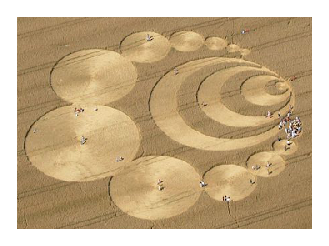
\includegraphics[width=5cm]{crop}
   \end{center}
   \bigskip
   \begin{cadre}[B2][F4]
      \begin{center}
         Vidéo : \href{https://www.francetvinfo.fr/replay-jt/france-2/20-heures/video-en-alsace-les-mysterieux-cercles-dans-le-champ-etaient-un-cours-de-maths_3505711.html}{\bf Les mystérieux cercles dans le champ étaient un cours de maths}, {\it franceinfo}, émission {\it L'Oeil du 20 h}.
      \end{center}
   \end{cadre}
\end{debat}

\vfill

\textcolor{PartieGeometrie}{\sffamily\bfseries Cahier de compétences} : chapitre 7, exercices 16 à 21 ; 25.


%%%%%%%%%%%%%%%%%%%%%%%%%%%%%%%%%%%%
%%%%%%%%%%%%%%%%%%%%%%%%%%%%%%%%%%%%
\activites

   \begin{activite}[Tracer des cercles avec GeoGebra]
      {\bf Objectif :} construire un point ; un cercle ; une figure complexe avec un logiciel de géométrie dynamique.
      \begin{QCM}
         Ouvrir Geogebra et choisir l'onglet \textbf{Géométrie}. \\
         \partie[placer un point et le renommer]
            Dans la barre d'outils, sélectionner le menu relatif aux points :
            \begin{pspicture}(-0.5,-0.5)(0.5,0)
               \psframe[framearc=0.2,linecolor=lightgray](-0.5,-0.5)(0.5,0.5)
               \psdot[linecolor=blue,linewidth=0.6mm](-0.15,-0.15)   
               \rput(0.15,0.15){\blue A}
            \end{pspicture} \\
            Choisir l'item \og Point \fg{} puis cliquer sur l'écran, que se passe-t-il ? \\ [1mm]
            \pf \\ [2mm]
            Déplacer le point grâce à l'outil \og Déplacer \fg :
            \begin{pspicture}(-0.5,-0.1)(0.5,.5)
               \psframe[framearc=0.2,linecolor=lightgray](-0.5,-0.5)(0.5,0.5)
               \pspolygon(0.15,-0.35)(0.26,-0.28)(0.01,0.1)(0.2,0.12)(-0.2,0.34)(-0.2,-0.12)(-0.1,0.03)
            \end{pspicture} \\

            Faire un clic droit sur le point et choisir \og Propriétés \fg. Changer le nom du point en O. \\
         
         \partie[tracer un cercle]
            Dans la barre d'outils, sélectionner le menu relatif aux cercles :
            \begin{pspicture}(-0.5,-0.5)(0.5,0)
               \psframe[framearc=0.2,linecolor=lightgray](-0.5,-0.5)(0.5,0.5)
               \psdots[linecolor=blue](0,0)(0.3;60)
               \pscircle(0,0){0.3}       
            \end{pspicture}. Que contient ce menu ? \\ [1mm]
                \pf \\ [2mm]
               \pf \\ [2mm]
            Il existe trois façons de tracer un cercle :
            \begin{center}
               \newcolumntype{M}{>{\itshape\footnotesize}p{5cm}}
               \begin{tabular}{|c|p{6cm}|p{2.5cm}|M|}
                  \hline
                  & Instructions & outil du menu & action \\
                  \hline
                  1 & \multicolumn{3}{l|}{On a le {\bf centre} et un {\bf point} du cercle} \\
                  \hdashline
                  & Placer un point O sur l'écran & Point & placer le point sur l'écran puis changer son nom \\
                  & Placer un point A sur l'écran & Point & placer le point sur l'écran puis changer son nom \\
                  & Tracer le cercle de centre O passant par A & Cercle\newline(centre-point) & sélectionner O, puis A \\
                  & Faire bouger A et O & Déplacer & sélectionner O ou A et les faire bouger \\
                  \hline
                  2 & \multicolumn{3}{l|}{On a le centre et le rayon du cercle} \\
                  \hdashline
                  & Placer un point B sur l'écran & & \\
                  & Tracer le cercle de centre B de rayon \ucm{3} & Cercle\newline(centre-rayon) & sélectionner B, puis entrer la valeur du rayon \\
                  & Faire bouger B & & \\
                  \hline
                  3 & \multicolumn{3}{l|}{On a trois points du cercle} \\
                  \hdashline
                  & Placer trois points C, L et E & Point & \\
                  & Tracer le cercle passant par C, L et E & Cercle (passant\newline par trois points) & sélectionner successivement, C, L et E \\
                  \hline
               \end{tabular}
            \end{center} \medskip
        
         \partie[défi !!!]
            Dessiner un bonhomme de neige : il est tout à fait possible d'explorer les autres menus de GeoGebra et de faire preuve de créativité. Le menu propriétés (clic droit) permet de colorier la figure ou de la remplir de motifs. \medskip
      \end{QCM}
   \end{activite}
   
   
%%%%%%%%%%%%%%%%%%%%%%%%%%%%%%%%%%%%
%%%%%%%%%%%%%%%%%%%%%%%%%%%%%%%%%%%%
\cours 

%%%%%%%%%%%%%%%%%%%%%%%%%%%%%%%%%%%%
\section{Le cercle, le disque}

\begin{definition}
   Le \textbf{cercle} de centre O de rayon $r$ est l'ensemble des points situés à une distance $r$ du point O. \\ 
   Le \textbf{disque} est l'intérieur du cercle.
\end{definition}

{\psset{unit=0.6}
\begin{pspicture}(-5,0.1)(10,4.9)
   \psdots(2,2)
   \rput(2,1.6){$O$}
   \psarc(2,2){2}{70}{-45}
   \psarc[linestyle=dashed](2,2){2}{-45}{70}
   \psline[linecolor=B1,arrowsize=0.25]{<->}(0,2)(2,2)
   \rput(1,2.3){\textcolor{B1}{$r$}}
   \rput(10,2){\begin{minipage}{3.2cm} Un cercle se dessine en général à l'aide d'un compas. \end{minipage}}
\end{pspicture}}

\begin{definition}
   \begin{itemize}
      \item Un {\bf rayon} d'un cercle est un segment d'extrémité le centre du cercle et un point du cercle, c'est aussi la longueur de ce segment.
      \item Une \textbf{corde} est un segment reliant deux points du cercle.
      \item Lorsqu'une corde passe par le centre du cercle, on l'appelle un \textbf{diamètre} du cercle.
      \item Une partie du cercle comprise entre deux points est appelée \textbf{arc} de cercle.
   \end{itemize}
\end{definition}

\begin{minipage}{9cm}
   \psset{unit=0.9}
   \begin{pspicture}(-3.5,0.2)(4,4.4)
      \psdots(2,2)
      \psarc[linecolor=A1](2,2){2}{180}{240}
      \psarc(2,2){2}{240}{180}
      \rput(2,1.6){$O$}
      \rput(0.4,3.7){$\mathcal{C}$}
      \psline[linecolor=B1](0,2)(2,2)
      \psdots(0,2)
      \rput(-0.3,2){$A$}
      \psdots(3,3.7)
      \rput(3.2,4){$B$}
      \psdots(1,0.3)
      \rput(0.8,-0.2){$C$}
      \psline[linecolor=D1](1,0.3)(3,3.7)
      \psline[linecolor=J1](0,2)(3,3.7)
      \psdots[dotstyle=+](1,2)(2.5,2.85)(1.52,1.2)
   \end{pspicture}
\end{minipage}
\begin{minipage}{7cm}
   \textcolor{B1}{$[OA]$ est un rayon du cercle $\mathcal{C}$.} \\
   \textcolor{D1}{$[BC]$ est un diamètre du cercle $\mathcal{C}$.} \\
   \textcolor{A1}{$\wideparen{AC}$ est un arc du cercle $\mathcal{C}$.} \\
   \textcolor{J1}{$[AB]$ est une corde du cercle $\mathcal{C}$.} \\[3mm]
   On a $OA = OB = OC$ et $BC =2\,OC$ \\
   $O$ est le milieu du segment $[BC]$
\end{minipage}


%%%%%%%%%%%%%%%%%%%%%%%%
\section{Rédiger un programme de construction}

Rédiger un programme de construction signifie écrire des instructions permettant de construire une figure.

\begin{exemple}
   Écrire un programme de construction permettant d'obtenir la figure ci-dessous puis la construire. \\   
   \small\psset{unit=0.5}
   \begin{pspicture}(0,-4)(12,4.5)
      \pscircle(2,0){2}
      \psarc(4,0){4}{0}{180}
      \psarc(8,0){4}{180}{0}
      \pscircle(10,0){2}
      \psdots(0,0)(4,0)(8,0)(12,0)
      \rput(0.4,-0.4){$A$}
      \rput(4.4,-0.43){$B$}
      \rput(8.4,-0.4){$C$}
      \rput(12.4,-0.4){$D$}
      \psline(0,0)(12,0)
      \rput(2,0.7){5 cm}
      \rput(2,0){/\!\!/}
      \rput(6,0){/\!\!/}
      \rput(10,0){/\!\!/}
   \end{pspicture}
   \correction
      - Tracer le segment $[AD]$ de longueur $AD =15$ cm. \\
      - Placer les points $B$ et $C$ sur ce segment tels que $AB =5$ cm et $AC =10$ cm. \\
      - Tracer le cercle de diamètre $[AB]$. \\ 
      - Tracer le demi-cercle de diamètre $[AC]$ situé au-dessus du segment $[AD]$. \\      
      - Tracer le demi-cercle de diamètre $[BD]$ situé en-dessous du segment $[AD]$. \\
      - Tracer le cercle de diamètre $[CD]$. \\ [2mm]
      {\it Attention : un programme de construction n'est pas unique et il ne mentionne pas les instruments à utiliser.}
\end{exemple}

   
%%%%%%%%%%%%%%%%%%%%%%%%%%%%%%%%%
%%%%%%%%%%%%%%%%%%%%%%%%%%%%%%%%%
\exercicesbase

\begin{colonne*exercice}

%%%%%
\serie{Vocabulaire du cercle}

\begin{exercice}
   Compléter les phrases suivantes en utilisant les mots : cercle - corde - rayon - centre - diamètre - milieu.
   \begin{itemize}
      \item Le \pfb ($\mathcal{C}_1$) de \pfb $E$ \\
         passe par les points $A, B, C, D$ et $F$.
      \item Le segment $[EF]$ est un \pf de ce cercle.
      \item Le segment $[AC]$ est une \pf de ce cercle.
      \item $E$ est le \pfb du \pfb $[AD]$.
   \end{itemize}
   \begin{center}
   \psset{unit=0.75}
   \begin{pspicture}(-2,-2.3)(2,2.5)
      \pstGeonode[PointSymbol=none,PosAngle={-135,80,140,220,-60,-40}]{E}(2;80){B}(2;140){A}(2;220){C}(2;-60){F}(2;-40){D}
      \pstCircleOA{E}{A}
      \pstSegmentMark{E}{A}
      \pstSegmentMark{E}{B}
      \pstSegmentMark{E}{D}
      \pstSegmentMark{E}{F}
      \pstLineAB{B}{C}
      \pstLineAB{A}{C}
      \rput(2.5;40){($\mathcal{C}_1$)}
   \end{pspicture}
   \end{center}
\end{exercice}

\begin{exercice}
   Compléter les phrases ci-dessous en utilisant la règle graduée ou le compas.
   \begin{itemize}
      \item Le cercle ($\mathcal{C}_1$) de centre J passant par G passe également par les points \pf et  \pf \\ [-5mm]
      \item Le cercle ($\mathcal{C}_2$) de centre P et de rayon PH passe par les points  \pf,  \pf et  \pf
      \item Les points  \pf,  \pf et  \pf sont sur \\
         le cercle ($\mathcal{C}_3$) de centre F et de rayon EF.
      \item Les points A, F et I sont sur le même cercle ($\mathcal{C}_4$) de centre  \pf
      \item Le point situé à l'intersection des cercles ($\mathcal{C}_2$) et ($\mathcal{C}_4$) est le point  \pf
   \end{itemize}
   \begin{center}
      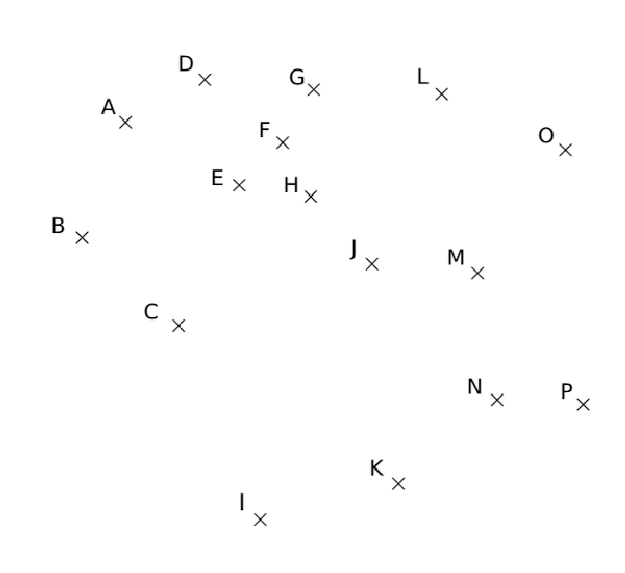
\includegraphics[width=8cm]{points}
   \end{center}
\end{exercice}

%%%%%
\serie{Programmes de construction}

\begin{exercice}
   Construire les figures suivantes :
   \begin{enumerate}
      \item
      \begin{itemize}
         \item Tracer un cercle ($\mathcal{C}$) de centre O et de rayon 4 cm puis un cercle de rayon 4 cm et passant par O.
         \item Où se trouve le centre du deuxième cercle ?
      \end{itemize}
      \item
      \begin{itemize}
         \item Tracer un segment [AB] de longueur 5 cm.
         \item Tracer le cercle ($\mathcal{C}$) de diamètre [AB].
         \item Quel est le rayon du cercle ($\mathcal{C}$) ?
      \end{itemize}
   \end{enumerate}
\end{exercice}

\begin{exercice}
   {\small Construire un carré} ABCD de côté 8 cm de centre O.
   \begin{itemize}
      \item Placer les points I, J, K et L milieux respectifs de [AB], [BC], [CD] et [DA].
      \item Sur ce carré, tracer chacun des cercles suivants :
      \begin{itemize}
         \item[-] ($\mathcal{C}_1$) de centre O passant par A.
         \item[-] ($\mathcal{C}_2$) de centre O et de rayon 2,5 cm.
         \item[-] ($\mathcal{C}_3$) dont [OD] est un diamètre.
      \end{itemize}
   \end{itemize}
\end{exercice}

\begin{exercice}
   Écrire un programme de construction pour chaque figure puis la construire. \\
   \psset{unit=0.6}
   \small
   \begin{pspicture}(-4,-2)(3,2.3)
      \pscircle(0,0){2}
      \psline{|-}(0,0)(2;45)
      \rput{45}(1,0.3){3,5 cm}
      \rput(-0.3,-0.3){P}
   \end{pspicture}
   \begin{pspicture}(-3,-2)(3,2.3)
      \pscircle(0,0){2}
      \psline{-}(2;180)(2;0)
      \psline[linecolor=gray]{<->}(2;175)(2;5)
      \rput(0,0.6){6,8 cm}
      \rput(0,-0.5){M}
      \rput(0,0){$\times$}
   \end{pspicture}
\end{exercice}

\begin{exercice}
   Écrire un texte pour décrire les différentes étapes de cette construction. \\
   \psset{unit=0.5}
   \footnotesize
   \begin{pspicture}(-3,-2.3)(3,2.3)
      \pscircle(0,0){2}
      \psline{-}(2;180)(2;0)
      \psline{<->}(2;175)(2;5)
      \rput(0,0.6){16 cm}
      \rput(0,-0.5){C}
      \rput(-2.5,0){A}
      \rput(2.5,0){B}
      \rput(0,0){$\times$}
      \rput(0,-2.7){étape 1}
   \end{pspicture}
   \begin{pspicture}(-3,-2.3)(3,2.3)
      \pscircle(0,0){2}
      \psline{-}(2;180)(2;0)
      \rput(-0.2,-0.5){C}
      \rput(1,-0.5){D}
      \rput(-2.5,0){A}
      \rput(2.5,0){B}
      \rput(0,0){$\times$}
      \rput(1,0){$\times$}
      \pscircle(1,0){1}
      \rput(0,-2.7){étape 2}
   \end{pspicture}
   \begin{pspicture}(-3,-2.3)(3,2.3)
      \pscircle(0,0){2}
      \psline{-}(2;180)(2;0)
      \rput(-0.2,-0.5){C}
      \rput(0.9,-0.5){D}
      \rput(-2.5,0){A}
      \rput(2.5,0){B}
      \rput(0,0){$\times$}
      \rput(1,0){$\times$}
      \pscircle(1,0){1}
      \pscircle(1.5,0){0.5}
      \rput(0,-2.7){étape 3}
   \end{pspicture}
\end{exercice}

%%%%%
\serie{Reproduire des figures}

\begin{exercice}
   Reproduire chaque figure sur le cahier. \\
   \psset{unit=0.25}
   \begin{pspicture}(-2,0)(14,16.5)
      \psgrid[griddots=20, subgriddiv=0, gridlabels=0,gridcolor=gray](-2,0)(14,16)
      \psarc(7,1){1}{180}{0}
      \psline(6,1)(6,8)
      \psline(0,10)(6,16)(12,10)
      \psline(4,10)(6,16)(8,10)
      \psarc(2,10){2}{180}{0}
      \psarc(6,10){2}{180}{0}
      \psarc(10,10){2}{180}{0}
   \end{pspicture}
   \begin{pspicture}(0,0)(16,16.5)
      \psgrid[griddots=20, subgriddiv=0, gridlabels=0,gridcolor=gray](0,0)(16,16)
      \psarc(3,3){2}{90}{0}
      \psarc(8,3){3}{0}{180}
      \psarc(13,3){2}{180}{90}
      \psarc(13,8){3}{90}{270}
      \psarc(13,13){2}{-90}{180}
      \psarc(8,13){3}{180}{0}
      \psarc(3,13){2}{0}{270}
      \psarc(3,8){3}{-90}{90}
   \end{pspicture}
\end{exercice}

\end{colonne*exercice}


%%%%%%%%%%%%%%%%%%%%%%%%%%%%%%%%%%%%
\Recreation

   \enigme[Rosaces]
      Dessiner une rosace (sur une feuille unie) puis la colorier et la découper. Elle peut par exemple ressembler à l'une des trois rosaces ci-dessous mais il est aussi possible de faire travailler son imagination !
   \begin{center}
      \begin{pspicture}(-4,-5)(4,5.5)
         \pscircle(0,0){4}
         \multido{\n=0+30,\i=120+30,\r=240+30}{12}{\psarc(4;\n){4}{\i}{\r}}
      \end{pspicture}
      \qquad
      \begin{pspicture}(-4,-5)(4,6)
         \multido{\n=0+30}{12}{\pscircle(2;\n){2}}
      \end{pspicture}
      \begin{pspicture}(-4,-4)(4,4)
         \pscircle(0,0){4}
         \pscircle(0,0){2}
         \pscircle(0,0){3.5}
         \multido{\n=0+60}{6}{\pscircle(2;\n){2}}
      \end{pspicture}
   \end{center}






